\paragraph{QuizziPedia::Front-End::Controllers::TrainingController}
\begin{figure} [ht]
	\centering
	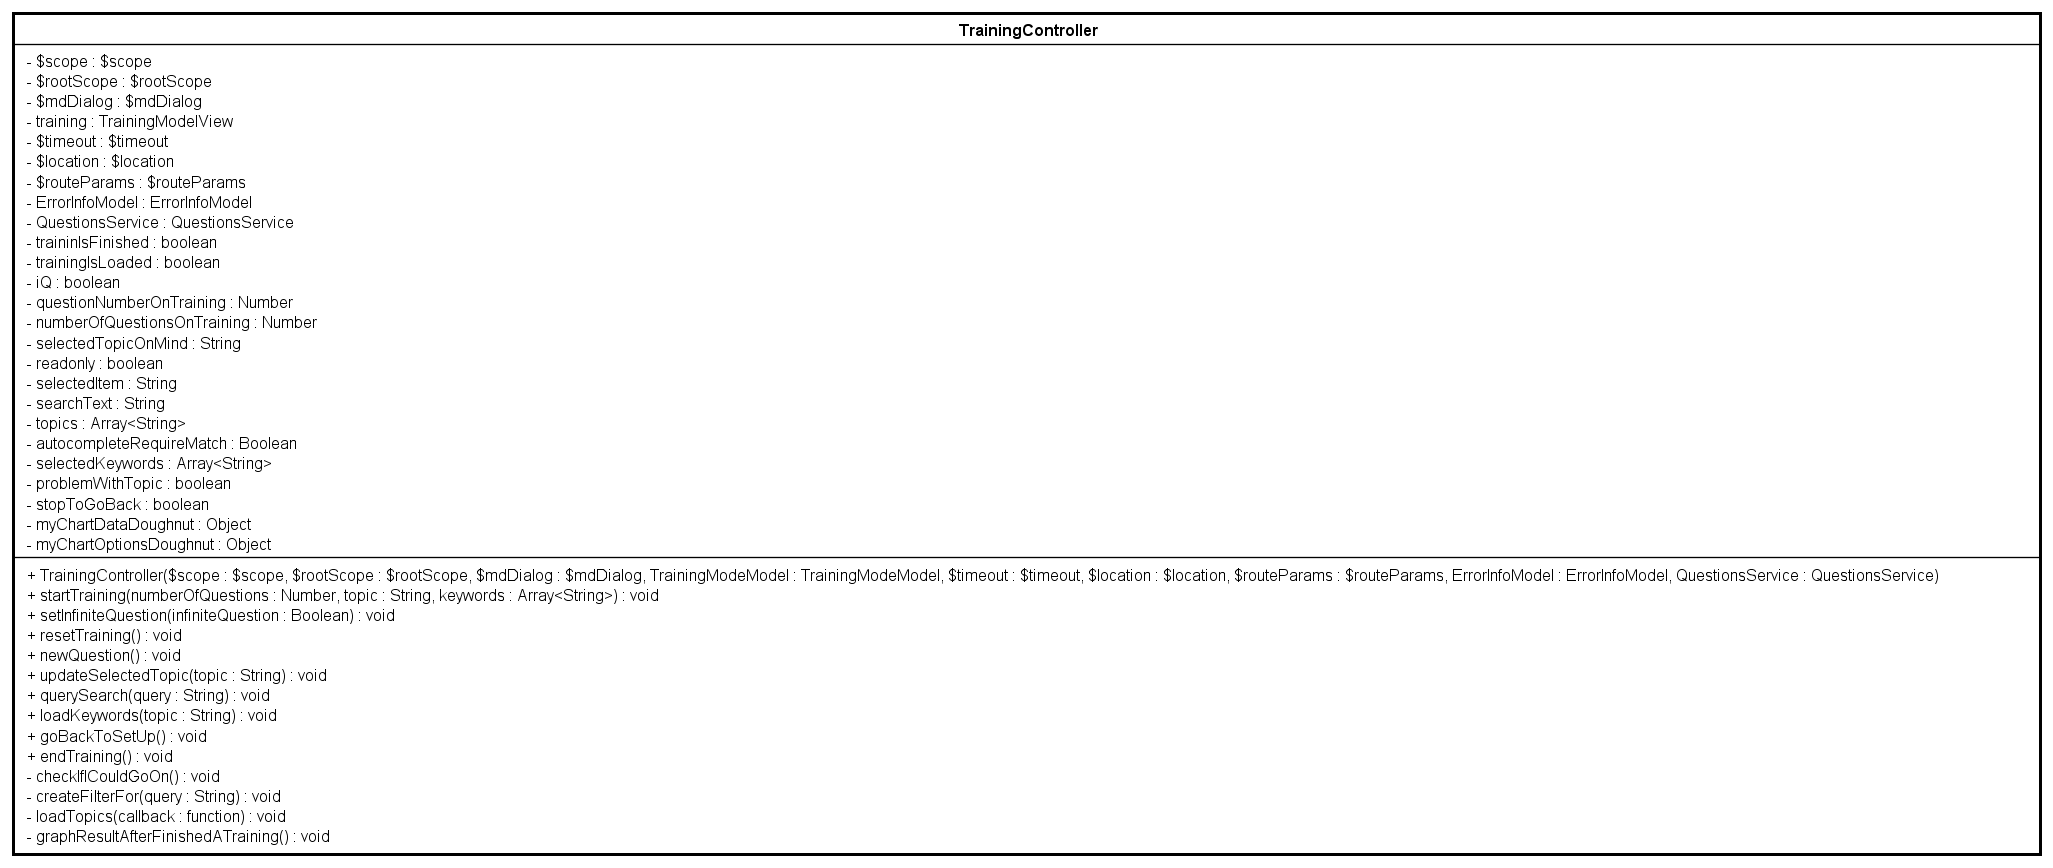
\includegraphics[scale=0.25]{UML/Classi/Front-End/QuizziPedia_Front-end_Controller_TrainingController.png}
	\caption{QuizziPedia::Front-End::Controllers::TrainingController}
\end{figure} \FloatBarrier
\begin{itemize}
	\item \textbf{Descrizione}: questa classe permette di gestire la modalità allenamento sottoponendo all'utente le giuste domande adatte al suo livello;
	\item \textbf{Utilizzo}: fornisce le funzionalità per recuperare le domande che siano in accordo con il livello dell'utente;
	\item \textbf{Relazione con altre classi}:
	\begin{itemize}
		\item \textbf{IN \texttt{TrainingModelView}}: classe di tipo \textit{modelview\ped{G}} la cui istanziazione è contenuta all'interno della variabile di ambiente \$scope di \textit{Angular\ped{G}}. All'interno di essa sono presenti le variabili e i metodi necessari per il \textit{Two-Way Data-Binding\ped{G}} tra la \textit{view\ped{G}} \texttt{TrainingView} e il \textit{controller\ped{G}} \texttt{TrainingController};
		\item \textbf{IN \texttt{TrainingModeModel}}: rappresenta un allenamento. Contiene tutte le informazioni necessarie alla presentazione del contenuto di un allenamento;
		\item \textbf{IN \texttt{QuestionController}}: questa classe permette di gestire il recupero delle domande per far si che possano essere visualizzate nella modalità allenamento e nella compilazione dei questionari.
	\end{itemize}
	\item \textbf{Attributi}:
	\begin{itemize}
		\item \texttt{-} \texttt{\$scope: \$scope} \\
		Campo dati contenente un riferimento all'oggetto \$scope creato da \textit{Angular\ped{G}}, viene utilizzato come mezzo di comunicazione tra il \textit{controller\ped{G}} e la \textit{view\ped{G}}. Contiene gli oggetti che definiscono il \textit{model\ped{G}} dell'applicazione;
		\item \texttt{-} \texttt{\$rootScope: \$rootScope} \\
		Campo dati contenente il riferimento all'oggetto globale \$rootScope creato da \textit{Angular\ped{G}}. Viene utilizzato per rendere accessibile a tutti i \textit{controller\ped{G}} e a tutte le \textit{view\ped{G}} l'oggetto \texttt{TrainingModeModel}. In questo caso viene utilizzato per inserire in \$rootScope l'oggetto di ritorno della chiamata a \texttt{getNextQuestion};
		\item \texttt{-} \texttt{\$mdDialog: \$mdDialog} \\
		Campo dati contenente un riferimento al servizio della libreria \textit{Material for Angular\ped{G}} che permette di creare delle componenti a pop-up;
		\item \texttt{+} \texttt{training: TrainingModelView} \\
		Oggetto di tipo \texttt{TrainingModelView}. All'interno di esso sono presenti le variabili e i metodi necessari per il \textit{Two-Way Data-Binding\ped{G}} tra la \textit{view\ped{G}} \texttt{TrainingView} e il \textit{controller\ped{G}} \texttt{TrainingController};
		\item \timeoutA;
		\item \locationA;
		\item \routeparamsA;
		\item \errorinfomodelA;
		\item \questionsserviceA;
		\item \texttt{-} \texttt{traininIsFinished: Boolean} \\Campo dati che indica se l'allenamento è terminato;
		\item \texttt{-} \texttt{trainingIsLoaded: Boolean} \\Campo dati che indica se l'allenamento è caricato;
		\item \texttt{-} \texttt{iQ: Boolean} \\Campo dati che indica se sono state scelte infinite domande;
		\item \texttt{-} \texttt{questionNumberOnTraining: Number} \\Campo dati che indica il numero progressivo della domanda attuale;
		\item \texttt{-} \texttt{numberOfQuestionsOnTraining: Number} \\Campo dati che il numero totale di domande;
		\item \texttt{-} \texttt{selectedTopicOnMind: String} \\Campo dati che tiene in memoria l'ultimo argomento scelto per l'allenamento. Utile per poter rifare l'allenamento;
		\item \texttt{-} \texttt{readonly: Boolean} \\Campo dati che indica se la form per l'inserimento delle parole chive è di sola lettura;
		\item \texttt{-} \texttt{selectedItem: String} \\Campo dati che indica l'argomento scelto;
		\item \texttt{-} \texttt{searchText: String} \\Campo dati che contiene il testo ricercato per trovare le parole chiavi;
		\item \texttt{-} \texttt{topics: Array<String>} \\Campo dati che contiene l'array degli argomenti presenti nel sistema;
		\item \texttt{-} \texttt{autocompleteRequireMatch: Boolean} \\Campo dati che permette l'autocompletamento nella ricerca delle parole chiavi;
		\item \texttt{-} \texttt{selectedKeywords: Array<String>} \\Campo dati che contiene le parole chiave selezionate;
		\item \texttt{-} \texttt{problemWithTopic: Boolean} \\Campo dati che indica se ci sono problemi nel riavvio del questionario;
		\item \texttt{-} \texttt{stopToGoBack: Boolean} \\Campo dati che blocca il ritorno alla pagina precedente durante l'allenamento. All'utente viene chiesto cosa fare;
		\item \texttt{-} \texttt{myChartDataDoughnut: Object} \\ Campo dati che rappresenta i dati che verranno mostrati nel grafico finale;
		\item \texttt{-} \texttt{myChartOptionsDoughnut: Object} \\ Campo dati che rappresenta le opzioni per la rappresentazione del grafico finale.
	\end{itemize}
	\item \textbf{Metodi}:
	\begin{itemize}
		\item \texttt{+} \texttt{TrainingController(\$scope: \$scope, \$rootScope: \$rootScope, \$mdDialog: \$mdDialog, TrainingModeModel: TrainingModeModel, \$timeout: \$timeout, \$location: \$location, \$routeParams: \$routeParams, ErrorInfoModel: ErrorInfoModel, QuestionsService: QuestionsService)} \\ Metodo costruttore della classe. \\
		\textbf{Parametri:}
		\begin{itemize}
			\item \texttt{\$scope: \$scope} \\
			Parametro contenente un riferimento all'oggetto \$scope creato da \textit{Angular\ped{G}}. Viene utilizzato come mezzo di comunicazione tra il \textit{controller\ped{G}} e la \textit{view\ped{G}}. Contiene gli oggetti che definiscono il \textit{viewmodel\ped{G}} e il \textit{model\ped{G}} dell'applicazione;
			\item \texttt{\$rootscope: \$rootscope}\\
			Parametro contenente il riferimento all'oggetto globale \$rootScope creato da \textit{Ang-\\ular\ped{G}}. Viene utilizzato per rendere accessibile a tutti i \textit{controller\ped{G}} e a tutte le \textit{view\ped{G}} l'oggetto \texttt{UserDetailsModel}. In questo caso viene utilizzato per aggiornare in \$rootScope l'oggetto che rappresenta l'utente autenticato all'interno dell'applicazione;
			\item \texttt{\$mdDialog: \$mdDialog} \\
			Parametro contenente un riferimento al servizio della libreria \textit{Material for Angular\ped{G}} che permette di creare delle componenti a pop-up;
			\item \texttt{TrainingModeModel: TrainingModeModel} \\ Rappresenta un allenamento. Contiene tutte le informazioni necessarie alla presentazione del contenuto di un allenamento;
			\item \timeoutP;
			\item \locationP;
			\item \routeparamsP;
			\item \errorinfomodelP;
			\item \questionsserviceP.
		\end{itemize}
		
		\item \texttt{+} \texttt{startTraining(numberOfQuestions: Number, topic: String, keywords:\\ Array<String>): void} \\
		Metodo che gestisce l'evento per iniziare l'allenamento. \\
		\textbf{Parametri}:
		\begin{itemize}
			\item \texttt{numberOfQuestions: Number} \\
			Parametro contenente il numero di domande per l'allenamento;
			\item \texttt{topic: String} \\
			Parametro contenente l'argomento dell'allenamento;
			\item \texttt{keywords: Array<String>} \\
			Parametro contenente un array di stringhe che rappresenta le keywords scelte per l'allenamento.
		\end{itemize}
		\item \texttt{+} \texttt{setInfiniteQuestion(infiniteQuestion: Boolean): void} \\
		Metodo che imposta infinite domande per l'allenamento. \\
		\textbf{Parametri}:
		\begin{itemize}
			\item \texttt{infiniteQuestion: Boolean} \\
			Parametro che indica se l'allenamento è a domande infinite o meno.
		\end{itemize}
		\item \texttt{+} \texttt{resetTraining(): void} \\
		Metodo che permette di ricominciare l'allenamento con gli stessi parametri; 
		\item \texttt{+} \texttt{newQuestion(): void} \\
		Metodo che emette l'evento per scaricare una nuova domanda in base ai parametri passati. Prima di farlo richiama \texttt{checkIfICouldGoOn}; 
		\item \texttt{+} \texttt{updateSelectedTopic(topic: String): void} \\
		Metodo che aggiorna l'argomento scelto. \\
		\textbf{Parametri}:
		\begin{itemize}
			\item \texttt{topic: String} \\
			Parametro contenente l'argomento dell'allenamento.
		\end{itemize}
		\item \texttt{+} \texttt{querySearch(query: String): void} \\
		Metodo che ricerca tra le parole chiave. \\
		\textbf{Parametri}:
		\begin{itemize}
			\item \texttt{query: String} \\
			Parametro contenente la stringa digitata fino a quel momento per effettuare una ricerca tra le parole chiave di un determinato argomento.
		\end{itemize}
		\item \texttt{+} \texttt{loadKeywords(topic: String): void} \\
		Metodo che scarica tutte le parole chiave per un determinato argomento. \\
		\textbf{Parametri}:
		\begin{itemize}
			\item \texttt{topic: String} \\
			Parametro contenente l'argomento dell'allenamento.
		\end{itemize}
		\item \texttt{+} \texttt{goBackToSetUp(): void} \\
		Metodo che resetta tutte le variabili e permette di ricominciare l'allenamento impostando nuovi valori; \\
		\item \texttt{+} \texttt{endTraining(): void} \\
		Metodo che fa terminare l'allenamento; \\
		\item \texttt{-} \texttt{checkIfICouldGoOn(): void} \\
		Metodo che controlla se può andare alla domanda successiva e lancia gli eventi per controllare la risposta e memorizzare i risultati; \\
		\item \texttt{-} \texttt{createFilterFor(query: String): void} \\
		Metodo che rende lowercase la stringa di ricerca. \\
		\textbf{Parametri}:
		\begin{itemize}
			\item \texttt{query: String} \\
			Parametro contenente la stringa digitata fino a quel momento per effettuare una ricerca tra le parole chiave di un determinato argomento.
		\end{itemize}
		\item \texttt{-} \texttt{loadTopics(callback: function): void} \\
		Metodo che scarica tutti gli argomenti presenti nel sistema. \\
		\textbf{Parametri}:
		\begin{itemize}
			\item \texttt{-} \texttt{callback: function} \\
			Parametro che indica una funzione da eseguire per ritornare i dati al chiamante.
		\end{itemize}
		
		\item \texttt{+} \texttt{\$on('addResult': String, callback: function): void} \\
		Metodo che gestisce l'evento per aggiornare i risultati dati alle domande. \\
		\textbf{Parametri}:
		\begin{itemize}
			\item \texttt{-} \texttt{'addResult': String} \\
			Parametro che indica su quale evento rimanere in ascolto;
			\item \texttt{-} \texttt{callback: function} \\
			Parametro che indica una funzione da eseguire.
		\end{itemize}
		\item \texttt{+} \texttt{\$on('saveTheQuestion': String, callback: function): void} \\
		Metodo che gestisce l'evento per aggiungere la domanda corrente a quelle già fatte dell'allenamento. \\
		\textbf{Parametri}:
		\begin{itemize}
			\item \texttt{-} \texttt{'saveTheQuestion': String} \\
			Parametro che indica su quale evento rimanere in ascolto;
			\item \texttt{-} \texttt{callback: function} \\
			Parametro che indica una funzione da eseguire.
		\end{itemize}
		\item \texttt{+} \texttt{\$on('updateTemporaryLevel': String, callback: function): void} \\
		Metodo che gestisce l'evento per aggiornare il livello temporaneo di un utente non autenticato. \\
		\textbf{Parametri}:
		\begin{itemize}
			\item \texttt{-} \texttt{'updateTemporaryLevel': String} \\
			Parametro che indica su quale evento rimanere in ascolto;
			\item \texttt{-} \texttt{callback: function} \\
			Parametro che indica una funzione da eseguire.
		\end{itemize}
		\item \texttt{+} \texttt{\$on('backToTheSetUpTraining': String, callback: function): void} \\
		Metodo che gestisce l'evento per tornare alla pagina delle impostazioni del questionario. \\
		\textbf{Parametri}:
		\begin{itemize}
			\item \texttt{-} \texttt{'backToTheSetUpTraining': String} \\
			Parametro che indica su quale evento rimanere in ascolto;
			\item \texttt{-} \texttt{callback: function} \\
			Parametro che indica una funzione da eseguire.
		\end{itemize}
		\item \texttt{+} \texttt{\$on('\$locationChangeStart': String, callback: function): void} \\
		Metodo che gestisce l'evento per tornare alla pagina precedente. \\
		\textbf{Parametri}:
		\begin{itemize}
			\item \texttt{-} \texttt{'\$locationChangeStart': String} \\
			Parametro che indica su quale evento rimanere in ascolto;
			\item \texttt{-} \texttt{callback: function} \\
			Parametro che indica una funzione da eseguire.
		\end{itemize}
		\item \texttt{-} \texttt{graphResultAfterFinishedATraining(): void} \\
		Metodo imposta le variabili per la visualizzazione del grafico finale. 
		
		
	\end{itemize}
\end{itemize}

